\documentclass[times, utf8, diplomski, english]{fer_eng}
\usepackage{pdfpages}
\usepackage{listings}
\usepackage{color}
\usepackage{natbib}
\usepackage{graphicx}
\usepackage{tikz}
\usepackage{pgfplots}
\usepackage{bm}
\usepackage{relsize}
\usepackage{subfigure}
\setcitestyle{numbers}
\setcitestyle{square}
\bibliographystyle{unsrtnat}
\lstset{
basicstyle=\fontsize{8}{11}\ttfamily,
breaklines=true,
backgroundcolor=\color{lightgray}
}
\usepackage{listofitems} % for \readlist to create arrays
\usetikzlibrary{arrows.meta} % for arrow size
\usetikzlibrary{positioning}

\tikzset{>=latex} % for LaTeX arrow head
\usepackage{xcolor}
\colorlet{myred}{red!80!black}
\colorlet{myblue}{blue!80!black}
\colorlet{mygreen}{green!60!black}
\colorlet{myorange}{orange!70!red!60!black}
\colorlet{mydarkred}{red!30!black}
\colorlet{mydarkblue}{blue!40!black}
\colorlet{mydarkgreen}{green!30!black}
\tikzstyle{node}=[thick,circle,draw=myblue,minimum size=22,inner sep=0.5,outer sep=0.6]
\tikzstyle{node in}=[node,green!20!black,draw=mygreen!30!black,fill=mygreen!25]
\tikzstyle{node hidden}=[node,blue!20!black,draw=myblue!30!black,fill=myblue!20]
\tikzstyle{node convol}=[node,orange!20!black,draw=myorange!30!black,fill=myorange!20]
\tikzstyle{node out}=[node,red!20!black,draw=myred!30!black,fill=myred!20]
\tikzstyle{connect}=[thick,mydarkblue] %,line cap=round
\tikzstyle{connect arrow}=[-{Latex[length=4,width=3.5]},thick,mydarkblue,shorten <=0.5,shorten >=1]
\tikzset{ % node styles, numbered for easy mapping with \nstyle
	node 1/.style={node in},
	node 2/.style={node hidden},
	node 3/.style={node out},
}
\def\nstyle{int(\lay<\Nnodlen?min(2,\lay):3)} % map layer number onto 1, 2, or 3
\def\layersep{1.5}
\def\nodesep{1}

\begin{document}

\thesisnumber{3028}

\title{Using Graph Neural Networks to Separate Haplotypes in Assembly Graphs}

\author{Filip Wolf}

\maketitle

% Ispis stranice s napomenom o umetanju izvornika rada. Uklonite naredbu \izvornik ako želite izbaciti tu stranicu.
\includepdf[pages=-]{"hr_0036510053_56.pdf"}

% Dodavanje zahvale ili prazne stranice. Ako ne želite dodati zahvalu, naredbu ostavite radi prazne stranice.
\zahvala{}

\tableofcontents

\chapter{Introduction}

Traditionally, the focus of \textit{de novo} genome assembly has always been on the reconstruction of an individual's genome from its numerous broken-up fragments obtained after sequencing \cite{de_novo2}. We will here, however, focus on a different application of \textit{de novo} genome assembly: haplotype separation. Every individual's genome is composed of both a mother's and a father's genome. Because we inherit both parent's chromosomes, the genetic material between them gets mixed up, but some regions stay together regardless in the form of genes. The term \textit{haplotype} refers both to these inherited regions, as well as to all of the genes of a single parent on a chromosome \cite{haplotype}. In this thesis, we will use the term haplotype in the latter sense. By separating the two haplotypes in a genome, we can determine which parent is responsible for what genes. This has a wide range of applications, from ancestry tests to finding hereditary diseases \cite{haplotype_usage}.         

We will try to do this using novel algorithms from the field of \textit{deep learning} (DL), which is itself a subfield of \textit{machine learning} (ML). Bioinformatics has long been dominated by algorithms that employ complex heuristics and expert knowledge to find solutions to the problems researchers face \cite{compeau_pevzner_2015}. This is however slowly changing. More and more research is being done using ML to solve problems in bioinformatics, foregoing the laborious process of feature engineering and extensive human intervention. First, ML was employed only for finding dense and abstract representations of genome features, but it later started to completely replace the previously mentioned algorithms. It has since contributed tremendously to the field and shows no signs of stopping, the most notable achievement being the solution to the protein folding problem which previously wasn't solvable for 50 years \cite{alphafold}. Still, there remains a long way to go before ML, and to an extent, DL, becomes completely standard within the field. Thus, this thesis is concerned with applying recent DL techniques in order to solve the problem of separating haplotypes in genomes. This could not only potentially improve existing solutions to the problem at hand and reduce the necessity for human expert intervention, but also bring bioinformatics to a wider range of people who may not necessarily have a deep understanding of genetics \cite{dl_bioinformatics}.

\section{Bioinformatics}

Bioinformatics is an interdisciplinary field of research that has had a tremendous impact on humanity in the last few decades. Since the completion of the Human Genome Project \cite{HGP1} \cite{HGP2}, the cost of sequencing a human genome has fallen exponentially. We can now reliably sequence a human genome for less than a \$1000 \cite{genome_cost}, all thanks to recent advances in sequencing technology, as well as accompanying algorithms. In Section \ref{subsec:the process of sequencing and assembly}, we will briefly explain the general pipeline of genome sequencing and assembly, while in Section \ref{subsec:file formats}, we will go through all the file formats used in this thesis for storing data	.

\subsection{The Process of Sequencing \& Assembly}
\label{subsec:the process of sequencing and assembly}

In an ideal world, we would extract a human genome in the form of DNA from a cell, input it into a \textit{sequencer}, and get a complete and accurate sequence of a DNA molecule as output with no \textit{base pairs}\footnote{The four base pairs that constitute DNA are: adenine, cytosine, guanine, and thymine.} missing, which we could immediately use for further studying. Unfortunately, this perfect process is not (yet) a reality and it is hard to predict when this might become so. Due to this, we have to make due with sequencers that can only output genomes in the form of thousands of fragmented \textit{reads}, in our case at a median length of between 15 - 25 kilobase pairs (kbp) long, with shorter read sequencers sequencing reads at lengths of around 150 base pairs (bp) long in a process called \textit{shotgun sequencing}. There are also ultra-long reads with a maximum length of around 1 Mbp with a median length of 75 kbp, but these are not used for our experiments, as they are also of a smaller precision, something which is crucial for the success of our application. An average genome is much longer than that, e.g. the yeast genome is around 12 Mb long \cite{yeast} and the human genome is around 6.4 Gb long \cite{human}, so after sequencing, we need to assemble these short reads into longer ones before going further into analysis.

This process of assembling shorter reads into larger structures, called \textit{contigs}, is called \textit{assembly}, depicted as steps one through three in Figure \ref{fig:genome assembly}. We can use the overlaps between sequences (step two in Figure \ref{fig:genome assembly}) to build graphs in which each read is represented with a node, and each overlap between reads is represented with an edge in the graph. An overlap can be described as a match between two reads' \textit{ends}, i.e. the read's prefix (start) and suffix (end), which can come in the form of a prefix - suffix or an suffix - prefix overlap. The length of this overlap can indicate a stronger similarity between two reads, and therefore a stronger link in the graph between them. After we have found enough strong overlaps, we can finally combine reads into contigs. Lastly, we are tasked with finding the longest possible path on this graph to connect the individual contigs and form a complete genome. We also need to orient them properly, depicted as step four in Figure \ref{fig:genome assembly}.

\begin{figure}
	\centering
	\includegraphics[width=0.95\textwidth]{images/genome_assembly.png}
	\caption[Genome assembly]{An illustration depicting the process of \textit{de novo} genome assembly in four steps. First, fragmented sequences are obtained after sequencing. Next, we find overlaps between the sequences. We then combine these overlaps into contigs, and finally, determine the contigs' orientation to create scaffolds. This illustration was inspired by \cite{baker_2012}.}
	\label{fig:genome assembly}
\end{figure}

\subsection{File Formats}
\label{subsec:file formats}

As a distinct subfield that combines computer science and genetics, bioinformatics uses multiple file formats that are unique to it. Mostly used for storing representations of genomic data, they offer us a simpler way to work genome sequences, as well as modify them. In the following sections, we will briefly describe these file formats, as well as state their usage in this thesis.

\subsubsection{FASTA \& FASTQ}
\label{subsubsec:fasta and fastq}

The most common file format encountered while working with genomic data is the FASTA format, designated by its .fasta or .fa file extension. It is a text-based format for storing nucleotide sequences and their information. Base pairs of amino acids are stored using letters (A - adenine, C - cytosine, G - guanine, T - thymine) in the form of a long sequence. Every sequence starts with a description line, which is designated with a ">" symbol at the start of the line. The description line can contain various information about the sequence, such as sequence name, sequence length, sequence statistics, etc. In our case, it specified the species and chromosome to which the sequences belonged to (Section \ref{sec:introduction}). After generating the reads for our data (Chapter \ref{ch:dataset}), the description contained data such as the read number, strand information (forward or reverse), position on the chromosome, length and the chromosome to which it belonged to, as well as if it was a mutated read or not. Sometimes, we may want to also store sequence quality information into a FASTA file. For this, we use a FASTQ file. FASTQ files are usually used for storing reads, but as the reads we use are simulated, there is no need to store quality information about them. In the following example, we can see a typical line of a FASTA file filled with short reads:
\begin{lstlisting}
>read=1,reverse,position=1004750-1015277,length=10527,NC_001139.9
AAGCTTGCAGATTTATTAACAGTTCAAACGAGTTTGGCTGATAATGCTCGTGCAGGTATTGATCGTACGTACGTAGCTACGTG
\end{lstlisting}

\subsubsection{CSV}
\label{subsubsec:csv}

After generating various information about our dataset, we would store it in a CSV (comma separated values) file. That way, it could be  more easily read by some of the tools we used for extracting data from reads (Section \ref{sec:technology stack}). A CSV file can be thought of as a table, where values in a row are separated with a comma sign. The file starts with a header with column names that are also separated with commas.

Another reason why we use the CSV file format is because of the Raven assembler (Section \ref{subsec:assembling the graph}) outputting a CSV file with information about sequence overlap lengths. This information is stored in the file in the following way. We start in a descending order of read name. A line with an even index number represents an original read, while a line with an odd index number represents a \textit{virtual} read, i.e. a \textit{reverse complement} or \textit{strand} of the original read. A reverse complement represents the same sequence as the original, but in reverse order and with the base pairs replaced with their complements (A - T, C - G). The original and the reverse complement essentially represent the same genomic data, but on different strands of the DNA, which are either a forward or backward strand. An example of such a file ican be seein in the following example:
\begin{lstlisting}
6549 [3274] LN:i:9216 RC:i:1,6412 [3206] LN:i:11360 RC:i:1,1,39678 8937 0 0.992832
6413 [3206] LN:i:11360 RC:i:1,6548 [3274] LN:i:9216 RC:i:1,1,39679 11081 0 0.992832
6647 [3323] LN:i:10656 RC:i:1,6638 [3319] LN:i:10224 RC:i:1,1,39680 10347 0 0.990291
6639 [3319] LN:i:10224 RC:i:1,6646 [3323] LN:i:10656 RC:i:1,1,39681 9915 0 0.990291
\end{lstlisting}
First, we have the index of the first read. Then, in square brackets, we have the index of the original first read\footnote{Each virtual read forms a pair with an original read.}. We then have some read information, followed by the second read with which the first one forms an overlap, along with its own information. Lastly, we have three fields that represent the overlap length, the weight of the overlap (not used in this thesis) and its score, measured in the percentage of the overlap match\footnote{Overlaps do not need to be perfect to be used successfully.}. Each line essentially represents an edge in our graph between two nodes. The first $n$ lines in the file, where $n$ is the number of reads, represent the overlap between the original and virtual read. They are then followed by all other overlaps.

\subsubsection{GFA}
\label{subsubsec:gfa}

Another important file Raven outputs is a Graphical Fragment Assembly (GFA)\footnote{https://gfa-spec.github.io/GFA-spec/GFA1.html} file. It contains similar information to the CSV file, but with some notable additions, namely, instead of just specifying read overlaps, it also contains the whole sequences it uses in the assembly process. It also includes the original read names specified before assembly that contain mutation information. Each line in the file starts with an identifier, all the different ones being listed in the following table:
\begin{center}
	\begin{tabular}{ |c|c| }
		\hline
		\textbf{Type} & \textbf{Comment} \\
		\hline
		\# & Comment \\
		\hline
		H & Header \\
		\hline
		S & Segment \\
		\hline
		L & Link \\
		\hline
		C & Containment \\
		\hline
		P & Path \\
		\hline
		W & Walk \\
		\hline
	\end{tabular}
\end{center}
For our purposes, the file only contained lines starting with the letters S and L. S denotes a segment (sequence) used in the assembly, along with most of its information that was present before assembly (this is notable because it is missing in the CSV file). The lines starting with an L contain lines about sequence overlaps in a similar manner to the CSV file, with the addition of overlap length and mutation information, the latter being crucial for specifying which parent's haplotypes we are connecting with the overlaps. An example of lines starting with an L is in the following example:
\begin{lstlisting}
L	read=4158,reverse,position=395590-406211,length=10621,NC_001139.9|mutated +	read=4884,reverse,position=383506-395832,length=12326,NC_001139.9|mutated + 101M
L	read=4832,forward,position=802633-815655,length=13022,NC_001139.9|mutated -	read=4165,reverse,position=793088-803478,length=10390,NC_001139.9|mutated + 733M
\end{lstlisting}
The S lines are important because we can use them to associate the GFA file with the CSV file. This is due to the fact that the read index of a true read in the CSV file is equal to the line index of a sequence in the GFA file divided by two. So for example, the read with the true index 346 in the CSV file is equal to the sequence in line 173 in the GFA file.

\subsubsection{Miscellaneous}

Aside from the mentioned file formats, we created numerous other files of our own that either didn't have a suffix, or simply ended with a \textit{.txt} extension, for easier reading and writing. Those files were of an unspecified format and contained temporary information abut graphs, such as overlap lengths, parent affiliation, and similar.

\section{Thesis Task}

The task we are presented with here is slightly different compared to standard genome assembly. Instead of just finding a path through the assembly graph in order to assemble a complete genome, we are instead tasked with removing edges in the graph that connect contigs belonging to different parents. By doing this, we are essentially separating the two haplotypes that constitute a genome. To give more insight into this, we will explain what graphs are and how we use them in the following section.

\begin{figure}
	\centering
	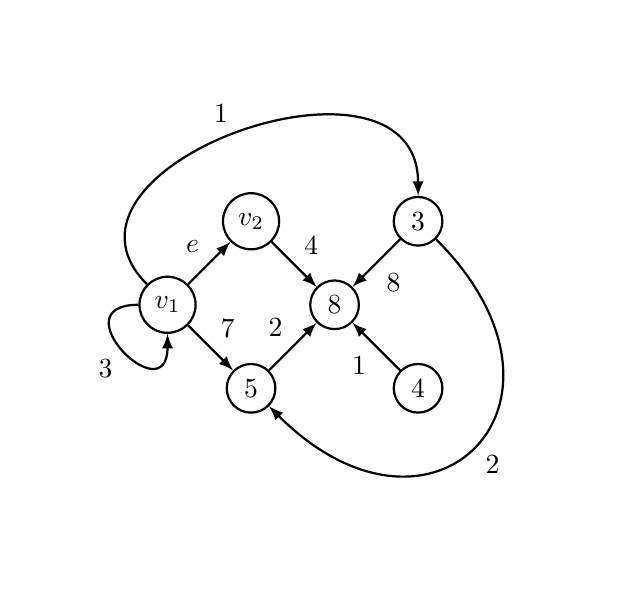
\begin{tikzpicture}[node distance={15mm}, thick, main/.style = {draw, circle}] 
	\node[main] (1) {$v_1$}; 
	\node[main] (2) [above right of=1] {$v_2$}; 
	\node[main] (3) [below right of=1] {5}; 
	\node[main] (4) [above right of=3] {8}; 
	\node[main] (5) [above right of=4] {3}; 
	\node[main] (6) [below right of=4] {4}; 
	\draw[->] (1) -- node[auto] {$e$} (2);
	\draw[->] (1) -- node[auto] {7} (3);
	\draw[->] (1) to [out=135,in=90,looseness=1.5] node[auto] {1} (5); 
	\draw[->] (1) to [out=180,in=270,looseness=5] node[auto, swap] {3} (1); 
	\draw[->] (2) -- node[auto] {4} (4); 
	\draw[->] (3) -- node[auto] {2} (4); 
	\draw[->] (5) -- node[auto] {8} (4); 
	\draw[->] (5) to [out=315, in=315, looseness=2.5] node[auto] {2} (3); 
	\draw[->] (6) -- node[auto] {1} (4); 
	\end{tikzpicture}
	\caption[Example graph]{An example of a directed graph with node and edge weights. Aside from every edge being directed, loops are also present, which connect nodes to themselves.}
	\label{fig:example_graph}
\end{figure}

\subsection{Graphs}

Graphs are data structures that can be defined with a set of nodes (vertices) $V$ and a set of edges connecting them $E$. Formally, this can be written as:
\[ G = (V, E) \]
where:
\[ E \subseteq 	\{ (x, y)|(x, y) \in V^2 \mathrm{\ and\ } x \neq y \} \]
The above definition is an example of a directed graph, meaning that the edges only go in one direction, which is the type of graph we work with in this thesis. A representation of such a graph can be seen in Figure \ref{fig:example_graph}. For instance, if edge $e$ is connecting nodes $v_1$ and $v_2$ in the direction $v_1 \rightarrow v_2$, then this means that node $v_1$ is connected to node $v_2$, but not the other way around. This is done so because edge direction can encode both suffix - prefix and prefix - suffix overlaps (Section \ref{subsec:the process of sequencing and assembly}), which is a useful information for us. Aside from this, both the nodes and edges have weights assigned to them that can represent various information about the graph \cite{trudeau_2017}.

In this thesis, after sequencing and assembly (Section \ref{subsec:the process of sequencing and assembly}), we obtain a list of reads connected to each other via overlaps. The reads can be thought of as nodes in a graph, while edges are the links between the nodes. By building such structures, we can more easily use existing graph theory insights to remove unwanted edges and separate the two haplotypes.

\section{Deep Learning}

In this section, we will go over the basics of deep learning (Section \ref{subsec:basics}), the main method behind the experiments in this thesis, followed with an overview of graph neural networks (Section \ref{subsec:graph neural networks}) and all the different variants of them we used. Lastly, in Section \ref{subsec:other functions}, we will explain all the different nonlinearities and regularization functions we used in our models.

\subsection{Basics}
\label{subsec:basics}

In the last decade, deep learning has grown from a niche research area to one of the most prominent fields withing computer science. It is now actively employed in virtually every human endeavor, from healthcare to entertainment \cite{dl_applications}. And it is still growing day by day on its mission to revolutionize the way we handle almost all data \cite{dl_growth}. To give insight into the field, will will explain the most basic building block of DL, Artificial Neural Networks, along with the algorithms that make them work: Stochastic Gradient Descent and Backpropagation.

\subsubsection{Artificial Neural Networks}

In deep learning, we use data processing structures called \textit{artificial neural networks} (ANNs) to extract information from data and learn to predict an outcome, such as some feature of the data or a target class to which the data belongs. An example of a fully connected neural network can be seen in Figure \ref{fig:neural network}. ANNs learn from data by adjusting trainable \textit{weights} that are defined for every connection between neurons in our network. Due to these weights, neural networks are much denser structures when compared to previous machine learning methods and can be referred to as \textit{universal function approximators} \cite{uni_approx} due to their ability to, with large enough networks, approximate any continuous function. This gives them unprecedented performance on previously unsolvable tasks, but due to their abstract structure, makes them somewhat difficult to interpret. Some networks, like \textit{convolutional neural networks} \cite{CNN}, don't suffer from this problem of interpretability as much and can produce some quite intuitive visualizations. On the other hand, some networks, like the ones we will use in this thesis, cannot be visually meaningfully interpreted. With all of this being said, how do ANNs actually work?

\begin{figure}
	\centering
	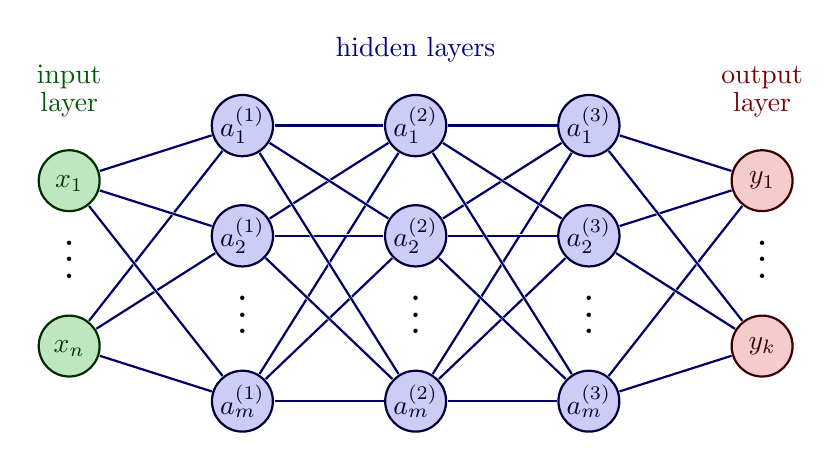
\begin{tikzpicture}[x=2.2cm,y=1.4cm]
		\readlist\Nnod{2,3,3,3,2} % array of number of nodes per layer
		\readlist\Nstr{n,m,m,m,k} % array of string number of nodes per layer
		\readlist\Cstr{\strut x,a^{(\prev)},a^{(\prev)},a^{(\prev)},y} % array of coefficient symbol per layer
		\def\yshift{0.5} % shift last node for dots
		
		\foreachitem \N \in \Nnod{ % loop over layers
			\def\lay{\Ncnt} % alias of index of current layer
			\pgfmathsetmacro\prev{int(\Ncnt-1)} % number of previous layer
			\message{\lay,}
			\foreach \i [evaluate={\c=int(\i==\N); \y=\N/2-\i-\c*\yshift;
				\index=(\i<\N?int(\i):"\Nstr[\lay]");
				\x=\lay; \n=\nstyle;}] in {1,...,\N}{ % loop over nodes
				% NODES
				\node[node \n] (N\lay-\i) at (\x,\y) {$\Cstr[\lay]_{\index}$};
				
				% CONNECTIONS
				\ifnum\lay>1 % connect to previous layer
				\foreach \j in {1,...,\Nnod[\prev]}{ % loop over nodes in previous layer
					\draw[connect,white,line width=1.2] (N\prev-\j) -- (N\lay-\i);
					\draw[connect] (N\prev-\j) -- (N\lay-\i);
					%\draw[connect] (N\prev-\j.0) -- (N\lay-\i.180); % connect to left
				}
				\fi % else: nothing to connect first layer
				
			}
			\path (N\lay-\N) --++ (0,1+\yshift) node[midway,scale=1.5] {$\vdots$};
		}
		
		% LABELS
		\node[above=0.2,align=center,mygreen!60!black] at (N1-1.90) {input\\[-0.2em]layer};
		\node[above=0.2,align=center,myblue!60!black] at (N3-1.90) {hidden layers};
		\node[above=0.2,align=center,myred!60!black] at (N\Nnodlen-1.90) {output\\[-0.2em]layer};
	\end{tikzpicture}
	\caption[Neural network]{Example of a fully connected neural network. Nodes represent individual artificial neurons. The green neurons represent the input to the network, which is of size $n$. The blue neurons represent the hidden layers, which are \textit{fully connected}, i.e. each neuron is connected to every other neuron in the previous and following layer. Each of these connections has a trainable weight associated with it used for learning how the neurons should pass data between them to learn from it. The hidden layers are of size $m$ with the numbers in brackets representing the layer index. Finally, the red neurons represent the output of the network, which is of size $k$. This image was taken from \cite{latex_nn}.}
	\label{fig:neural network}
\end{figure}

\subsubsection{Loss Function \& Stochastic Gradient Descent}
\label{subsubsec: loss function and stochastic gradient descent}

To successfully explain how ANNs work, we need to introduce two novel concepts: a loss function and the backpropagation algorithm. When we use a deep learning model to learn from data, we pass the data through our network and compare the output to a previously defined true value by using a \textit{loss function}. A loss function condenses the error of our network prediction to a single number which is then used to calculate gradients in respect to our data. The loss function we used for training models is described in more detail in Section \ref{subsec:loss function}. These gradients are then propagated back through the network using the \textit{backpropagation} algorithm. But, before explaining the backpropagation algorithm, we first need to explain a related, but simpler concept in the form of \textit{Stochastic Gradient Descent} (SGD). SGD is used for finding a function's minimum value. It accomplishes this by simply nudging all the variables (weights) of the function in the direction opposite the function's gradients. This will bring the weights closer to an optimal position for finding the minimum, as the gradient points in the opposite direction of the function minimum. This is represented in the following equation:
\[ w = w - \frac{\eta}{n} \sum_{i=1}^n \nabla Q_i(w) \]
where $w$ are the function weights, $n$ is the number of data samples, $\eta$ is the learning rate (Section \ref{subsec:optimizer}) and $\nabla Q_i(w)$ are the gradients of the function $Q$ in respect to weights $w$.

SGD can come in multiple forms. Standard SGD, as represented in the above equation, calculates these weight changes by first calculating function loss on all data we have available, averages it and only then updates weights. This method is very accurate, but also rather slow. On the other end of the spectrum, we can update weights after we process every piece of data, in what is called \textit{true} stochastic descent. This is very fast and has a lower chance of ending up in local optima, but is also too imprecise for fine-tuning function gradients during later stages of optimization. Due to this, we use a compromise between the two in the form of \textit{mini-batch} gradient descent. Instead of using only one data point or all data, we use a batch of data. Using larger batches is slower and more precise, while using smaller batches is faster and less precise. With that being said, we are most often limited by memory constraints while determining batch size and simply chose the largest batch size we can. Details about batch size in our model can be found in Section \ref{subsec:hyperparameters}.

\subsubsection{Backpropagation}
\label{subsubsec:backpropagation}

We can now move on to explaining the backpropagation algorithm. In essence, it is the idea of SGD applied to neural networks. It tells every weight in our network how to change in order to better predict our data. By correctly propagating these gradient values back through the network, we can successfully make our network learn from data. We will here briefly explain the theoretical background for backpropagation without going into too much detail.

After we obtain a loss value and calculate gradients, we need to somehow pass them back through the network and adjust network weights in accordance with the gradients. The way to do this is different depending on the layer of the network, but can be generally calculated using the partial derivative of the network error function (Section \ref{subsec:loss function}) in respect to the weights with the chain rule:
\[ \frac{\partial E}{\partial w_{ij}} = \frac{\partial E}{\partial o_j} \frac{\partial o_j}{\partial w_{ij}} = \frac{\partial E}{\partial o_j} \frac{\partial o_j}{\partial net_j} \frac{\partial net_j}{\partial w_{ij}}\]
Here, $E$ is the error of our network, $o_j$ is the output of layer $j$, $net_j$ is the output of layer $j$ before the activation function, and $w_{ij}$ is the weight of the neuron $i$ in layer $j$. Only one term in $net_j$ depends on $w_{ij}$, so we can substitute the last term in the above equation with $o_i$. If the neuron is in the output layer (denoted in a red color in Figure \ref{fig:neural network}), then $o_j = y$, so $\frac{\partial E}{\partial o_{j}} = \frac{\partial E}{\partial y}$. If it is in a hidden layer (denoted with a blue color in Figure \ref{fig:neural network}), the derivative is less obvious and we won't go into detail on how to obtain it, but will simply state it.

Finally, we get:
\[ \frac{\partial E}{\partial w_{ij}} = \delta_j o_i \]
where:
\[ \delta_j = \frac{\partial E}{\partial o_j} \frac{\partial o_j}{\partial net_j} = \begin{cases}
	\frac{\partial E}{\partial y} \frac{\partial \phi(net_j)}{\partial net_j} & \text{if $j$ is an output neuron,} \\
	(\sum_{l \in L} w_{jl} \delta_l) \frac{\partial \phi(net_j)}{\partial net_j} & \text{if $j$ is a hidden neuron.}
\end{cases}
\]
Here, $\phi$ is the activation function (Section \ref{subsubsec: nonlinearities}) and $L$ is the set of all neurons receiving input from neuron $j$, or in other words, all successor neurons to neuron $j$. Intuitively, a neuron's error depends on the error of all the neurons to which it passes its output. After we have obtained these values, we use the gradient descent method from the previous chapter to finally update network weights \cite{Goodfellow-et-al-2016}.

\subsection{Graph Neural Networks}
\label{subsec:graph neural networks}

While standard ANNs are great at predicting simple data with no underlying structure (or at least one that isn't known), to successfully make our network learn from assembly graphs, we will need something more refined. Although we can simply represent our graph in the form of a 1-dimensional vector by concatenating all the node and edge information, we this way lose precious structural information about contig overlaps. By using networks more tailor-made for data representation on graphs, we can take advantage of the graph's underlying structure. The networks in question are called \textit{Graph Neural Networks} (GNNs) \cite{GNN}. Most modern graph neural networks work on the principle of \textit{message passing} \cite{message_passing}. A node accumulates information from adjacent nodes and the edges connecting them and uses it to update its own weights. The information is represented in the form of node and edge features, multidimensional vectors of data that represent some information about the nodes and edges. By repeating this message passing process enough times, we can converge to a stable solution in which the network has learned something about the graph that was previously unseen to us. This can be formalized with following definition.

In graph $\mathcal{E}$, let $x_v \in \mathbf{R}^{d_1}$ be the features for node $v$, $w \in \mathbf{R}^{d_2}$ be the features for edge ($u$, $v$), and $m$ be a message generated by aggregating adjacent node information. The message passing paradigm defines the following edge-wise and node-wise computations at step $t+1$:
\[ \textrm{Edge-wise: } m_e^{(t+1)} = \phi (x_v^{(t)}, x_u^{(t)}, w_e^{(t)}), (u, v, e) \in \mathcal{E} \]
\[ \textrm{Node-wise: } x_v^{(t+1)} = \psi (x_v^{(t)}, \rho (\{m_e^{(t+1)}, \forall e \in \mathcal{N}(v))), (u, v, e) \in \mathcal{E} \]
In the above equations, $\phi$ is a \textit{message function} defined on each edge to generate a message by combining the feature $w_e^{(t)}$ of edge $e$ with the features of its incident nodes $x_v^{(t)}$ and $x_u^{(t)}$. Here, $t$ describes that the features are from step $t$. $\psi$ is an \textit{update function} defined on each node to update the features $x_v$ of node $v$ by aggregating messages coming from adjacent nodes in its neighborhood $\mathcal{N}$ using the \textit{reduce function} $\rho$.

\subsubsection{GNNs \& CNNs}

The GNN can be though of as an extension of CNNs. A CNN takes an image's local neighborhood and extracts information from it. It does this using convolutional \textit{filters}, which take a certain amount of pixels in a neighborhood and multiply them with weights. Now, the size of this filter is predefined and cannot be changed. For instance, it can have a size of 3 x 3 or 5 x 5. If we were to create such a filter for use in graphs, we would simply designate the central weight of the filter to be the node we are currently looking at, and the surrounding weights would be its neighboring nodes. As we can see, this would limit us to graphs where nodes had a constant number of neighbors, or graphs where we could look only at a limited number of neighbors. GNNs do not have this limitation, as the update function $\psi$ takes all nodes in a central node's neighborhood into account equally \cite{GRL} \cite{bronstein2021geometric}.

\begin{figure}
	\centering
	\includegraphics[width=\textwidth]{images/gnn_backprop.png}
	\caption[GNN backpropagation]{A diagram depicting the process of unfolding a graph in order to calculate its gradients. In the first step (top), we can see a graph. We then build a network in terms of the graph's update functions $g$ and $f$, thereby obtaining an encoding network corresponding to our graph. In the last step (bottom), we unfold the encoding network to get a recurrent neural network where each layer contains all of the graph's functions $f$ and $g$ and defines how they pass values between them. We than apply backpropagation on recurrent neural networks. Image taken from \cite{GNN}.}
	\label{fig:gnn backprop}
\end{figure}

\subsubsection{Backpropagation for GNNs}

Calculating backpropagation for GNNs is somewhat different from regular backpropagation described in Section \ref{subsubsec:backpropagation}. We will here try to explain it intuitively without going into too much mathematical detail, as it's beyond the scope of this thesis and rather unnecessary for understanding how GNNs work. First, it is necessary to look at a GNN as consisting of units of functions $\phi$ and $\psi$, which were described in the previous section. We can then build a network of these functions that corresponds to our graph called an \textit{encoding network}. When functions $\phi$ and $\psi$ are implemented as regular neural networks, the encoding network turns out to be a \textit{recurrent neural network}, i.e. a time dependent network whose neurons take as input values from a previous neuron and themselves. After we unfold this network, we get a time series that corresponds to steps in our GNN learning process. Each of these steps contains all of the units (functions $\phi$ and $\psi$) in an encoding network and defines how they pass messages to each other in each time step. We then apply backpropagation on recurrent neural networks, as defined in \cite{rnn_backprop}. This process can be seen in Figure \ref{fig:gnn backprop} \cite{GNN}.

We used three different GNNs in this thesis, which we will describe in the following sections. We will start with the most basic GNN we used, the Graph Convolutional Network (Section \ref{subsubsec:graph convolutional netwroks}), follow it up with Graph Attention Networks (Section \ref{subsubsec:graph attention networks}) which employ the attention mechanism to improve performance, and finally finish with the most complex network type, the Edge Graph Attention Network (Section \ref{subsubsec:edge graph attention network}) which incorporates the attention mechanism on both edges and nodes.

\subsubsection{Graph Covolutional Networks}
\label{subsubsec:graph convolutional netwroks}

The first network we used was the simplest and oldest one, and it bases its computations on Graph Convolutional Networks (GCN) \cite{GCN}. It aggregates information from neighboring nodes and the edges connecting them and uses them to update the central node's information. It updates node features with the following equation:
\[ h_i^{(l+1)} = \sigma \left(b^{(l)} + \sum_{j \in \mathcal{N}(i)} \frac{e_{ji}}{c_{ji}} h_j^{(l)} W^{(l)} \right) \]
where:
\[ c_{ji} = \sqrt{|\mathcal{N}(j)|} \sqrt{|\mathcal{N}(i)|} \]
Here, $\mathcal{N}(i)$ represents all the neighboring nodes of node $i$, $e_{ji}$ is the scalar weight of the edge connecting nodes $i$ and $j$, and $\sigma$ is an activation function. $b^{(l)}$, $h_j^{(l)}$ and $W^{(l)}$ are the networks bias at step $l$, features of node $j$ at step $l$ and weight of the network at step $l$ respectively. The aggregated information is used to update the features $h$ of node $i$ at step $(l+1)$. We can see that the calculations used are fairly straightforward, as we simply multiply the network weight and node features and add bias before passing it through a nonlinearity. A reader familiar with deep learning may notice that this is similar to an iteration of the backpropagation algorithm, but applied to the graph domain.

\subsubsection{Graph Attention Networks}
\label{subsubsec:graph attention networks}

The second network we used is more complex than a simple GCN, as it uses the \textit{attention mechanism} \cite{attention} to improve its performance. The Graph Attention Network (GATv2) \cite{GATv2} we used is an updated version of the original GAT \cite{GAT}, and we did notice a slight increase in performance while using it. It's node feature update function can be defined as:
\[ h_i^{(l+1)} = \sum_{j \in \mathcal{N}(i)} \alpha_{ij}^{(l)} W_{right}^{(l)} h_j^{(l)} \]
where:
\[ \alpha_{ij}^{(l)} = \mathrm{softmax}_i (e_{ij}^{(l)}) \]
\[ e_{ij}^{(l)} = \vec{a}^{T^{(l)}} \mathrm{LeakyReLU} (W_{left}^{(l)} h_i + W_{right}^{(l)} h_j) \]
Here, $W_{right}$ is one of the two network weight matrices, $h$ is a node feature matrix, $\alpha$ is an attention weight and $\vec{a}$ is the attention weight vector, which is also trainable. We can see that the basic equation is similar to the GCN, but with an added attention weight. This weight is the main reason why the network performs better compared to the regular GCN. The attention mechanism works by selecting data instances during training, such as graph nodes, that it considers more important than other data and thereby gives it more weight. This way, it increases model capacity and performance, while at the same time not directly increasing the network size. It is also worth mentioning that we can specify a number of \textit{attention heads} used in the attention mechanism. Attention heads are simply multiple attention mechanisms at work at the same time. The final attention score is calculated by concatenating or averaging these different attention values. This is done to improve training stability and, ultimately, performance.

This network differs from the original GAT only in the way $e_{ij}^{(l)}$ is calculated. Instead of using a single weight matrix $W$ that is concatenated to the features $h$, we use two separate matrices in the form of $W_{right}$ and $W_{left}$, giving the network more parameters and learning power.

\subsubsection{Edge Graph Attention Network}
\label{subsubsec:edge graph attention network}

The last network we used, and by far the most effective one, is a graph attention layer that handles edge features along with node features called Edge Graph Attention Network (EGAT) \cite{EGAT}. The main update equation is the same as in a GAT, but the difference lies in how the attention scores $e_{ij}$ are calculated. Instead of the usual way, they are obtained like the following:
\[ e_{ij} = \vec{a} f_{ij}^{'} \]
\[ f_{ij}^{'} = \mathrm{LeakyReLU} (A[h_i||f_{ij}||h_j]) \]
Here, $f_{ij}$ represents edge features, $A$ is a weight matrix and $\vec{a}$ is a weight vector. This network greatly improves performance due to the fact that it better utilizes edge features. Instead of just using them as weights to scale edge importance, it handles them in the same manner of importance as node features. This way, the network can find meaning in the edge weights much better compared to a regular GAT network. It is also worth noting that, compared to the other GNN layers described here, the EGAT layer returns both updated node and edge features, which then need to be handled further in the network.

\subsection{Other Functions}
\label{subsec:other functions}

In this section, we will explain all the functions we use in our networks that aren't directly responsible for training, but instead help in it, such as regularization functions and nonlinearities.

\begin{figure}
	\centering
	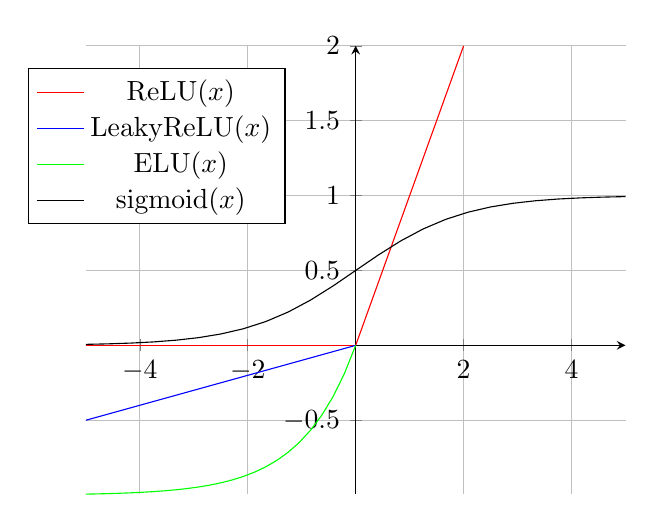
\begin{tikzpicture}
		\begin{axis}
		[
		grid=major,
		axis x line=middle,
		axis y line=middle,
		domain=-5:2,
		legend style={at={(0.37,0.95)}}  
		]
			\addplot+[mark=none,red,domain=-5:0] {0};
			\addplot+[mark=none,red,domain=0:2] {x};
			\addplot+[mark=none,blue,domain=-5:0] {0.1*x};
			\addplot+[mark=none,green,domain=-5:0] {exp(x)-1};
			\addplot+[mark=none,black,domain=-5:5] {1/(1+exp(-x))};
			\legend{$\mathrm{ReLU}(x)$,,$\mathrm{LeakyReLU}(x)$,$\mathrm{ELU}(x)$, $\mathrm{sigmoid}(x)$}
		\end{axis}
	\end{tikzpicture}
\caption{An example of all the different nonlinearities used in this thesis for model training. In red, we can see a regular ReLU function, which is valued at zero for $x<0$. The blue line represents the LeakyReLU function, which lets a small value pass through it for $x<0$, here valued at $0.1*x$. For $x>0$, it is the same as the ReLU. The green line represents the ELU function, which takes an exponential form for $x<0$ and is also the same as the ReLU for $x>0$. We can observe that these functions are different only for $x<0$. Lastly, the black line represents the sigmoid function. Unlike the other functions, it restricts both positive and negative values to a range of $[0,1]$.}
\label{fig:nonlinearities}
\end{figure}

\subsubsection{Nonlinearities}
\label{subsubsec: nonlinearities}

We use four different nonlinearities in our work. Three of them are used as nonlinearities between network layers, and one of them, the sigmoid function, is used for the final classification of graph edges. First, we are going to describe the network nonlinearities. The most basic one is the \textbf{ReLU} (Rectified Linear Unit) \cite{relu}, represented with the red line in Figure \ref{fig:nonlinearities}. It can be described with the following equation:
\[ \mathrm{ReLU}(z) = \max (0, z) \]
In other words, it passes through everything that is positive in a linear fashion, and sets everything else to zero. This is one of the most widely used nonlinearities and oldest ones. It has the same benefits as a sigmoid function or a tanh function (being differentiable), but is less computationally expensive and doesn't suffer from the saturation problem for high input values like the sigmoid does. That being said, it does suffer from the exploding gradients problem because, unlike the sigmoid or tanh, it does not restrict the size of positive outputs.

A variant of the ReLU is the \textbf{LeakyReLU} \cite{leakyrelu}, represented with the blue line in Figure \ref{fig:nonlinearities}. It only differs from ReLU in that it allows for a small non-zero constant gradient $\alpha$ to be passed through below zero. It does this in order to try to fix a limitation of ReLU where some neurons never express their values due to them always being negative, meaning that the ReLU never lets their values pass through.

Finally, we have the \textbf{ELU} (Exponential Linear Unit) \cite{elu}, represented with the green line in Figure \ref{fig:nonlinearities}. It can be described with the following equation:
\[ \mathrm{ELU}(z) = \begin{cases} 
z & z > 0 \\
\alpha \cdot (e^z - 1) & z \leq 0
\end{cases} \]
For values greater than 0, it emits a linear output just like the ReLU. But for any other value, it slowly smooths out bellow zero where it tends to the value of $- \alpha$. Just like LeakyReLU, it also tries to negate the previously mentioned weakness of ReLU. Both the ELU and the LeakyReLU can be used as strong alternatives to to the ReLU.

Lastly, for the classification of the network outputs, we need to normalize them into a $[0, 1]$ range so that they can be interpreted as probabilities. For this, we use the \textbf{sigmoid} function, represented with the black line in Figure \ref{fig:nonlinearities} and described with the following equation:
\[ S(x) = \frac{1}{1 + e^{-x}} \]
where $x$ is the input to the function. It is worth noting that for cases where there are more than two classes present, we actually use the \textit{softmax} function, described with the following equation:
\[ \sigma(x) = \frac{\exp (x_i)}{\sum_j \exp (x_j)} \]
The sigmoid is essentially just a special case of the softmax function for just two classes.

\subsubsection{Regularization Functions}
\label{subsubsec:regularization functions}

We used three different regularization functions throughout the networks we tested. In general, these functions help stabilize and speed up network training, as well as often improve performance.

Before imputing our data into the model, we need to \textbf{normalize} it, i.e. bring its values into a $[0,1]$ range. This is done so that input data from different sources is all in the same range. If this isn't done automatically in the network, we do it with built-in functions. There are many different ways to normalize edge and node data. For node features, we used input and output node degrees, which are normalized by subtracting the minimal respective node degree value from them and dividing them with the maximum value which was also reduced with the minimal value, a process known as min-max scaling. Formally, this can be written as:
\[ x' = \frac{x - \min(x)}{\max(x) - \min(x)} \]
Normalizing edge weights is a bit more complicated. The method we use for this is represented with the following equation:
\[ c_{ji} = \left( \sqrt{\sum_{k \in N(j)} e_{jk} } \sqrt{\sum_{k \in N(i)} e_{ki} } \right) \]
where $e_{jk}$ and $e_{ki}$ are the weights of the edges from node $j$ to node $k$ and from node $k$ to node $i$ respectively. We divide all weights with weight $c_{ji}$ to normalize them. Intuitively, what we do is multiply the square roots of the sums of weights of the edges connected to the two nodes that are being connected by edge $e_{ji}$. It is worth noting that we usually did not use node degree normalization, as we would transform the node data into a higher abstract dimension using a fully connected neural network anyway, in which case the individual node degrees would get lost.

\begin{figure}
	\centering
	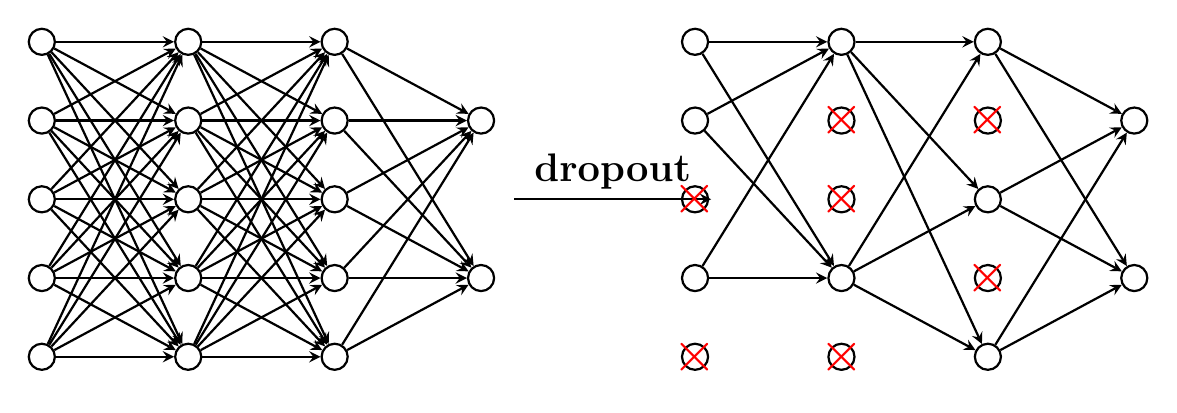
\begin{tikzpicture}[
	node/.style={circle, draw, thick},
	]
	
	\foreach \y in {1,...,5}{
		\node[node] (i\y) at (0,\nodesep*\y) {};
		\node[node, right=\layersep of i\y] (h1\y) {};
		\node[node, right=\layersep of h1\y] (h2\y) {};
	}
	
	\node[node, right=\layersep of h22] (o1) {};
	\node[node, right=\layersep of h24] (o2) {};
	
	\foreach \source in {1,...,5}
	\foreach \dest in {1,...,5}{
		\path[-stealth, thick] (i\source) edge (h1\dest);
		\path[-stealth, thick] (h1\source) edge (h2\dest);
	}
	\foreach \source in {1,...,5}
	\foreach \dest in {1,2}
	\draw[-stealth, thick] (h2\source) -- (o\dest);
	
	\draw[-stealth, thick] (6, 3*\nodesep) -- node[above,font=\Large\bfseries] {dropout} (8.5, 3*\nodesep);
	
	% Boundary
	
	\foreach \y in {1,...,5}
	\node[node, right=12em of h2\y] (di\y) {};
	
	\node[red,font=\huge] at (di1) {$\times$};
	\node[red,font=\huge] at (di3) {$\times$};
	
	\foreach \y in {1,...,5}
	\node[node, right=\layersep of di\y] (dh1\y) {};
	
	\node[red,font=\huge] at (dh11) {$\times$};
	\node[red,font=\huge] at (dh13) {$\times$};
	\node[red,font=\huge] at (dh14) {$\times$};
	
	\foreach \y in {1,...,5}
	\node[node, right=\layersep of dh1\y] (dh2\y) {};
	
	\node[red,font=\huge] at (dh22) {$\times$};
	\node[red,font=\huge] at (dh24) {$\times$};
	
	\node[node, right=\layersep of dh22] (do1) {};
	\node[node, right=\layersep of dh24] (do2) {};
	
	\foreach \source in {2,4,5}
	\foreach \dest in {2,5}
	\draw[-stealth, thick] (di\source) -- (dh1\dest);
	
	\foreach \source in {2,5}
	\foreach \dest in {1,3,5}
	\draw[-stealth, thick] (dh1\source) -- (dh2\dest);
	
	\foreach \source in {1,3,5}
	\foreach \dest in {1,2}
	\draw[-stealth, thick] (dh2\source) -- (do\dest);
	
	\end{tikzpicture}
	\caption{An example of dropout. The network on the left is fully connected, while on the network on the right, we can see that some nodes, as well as their connections, have been dropped. This leads to a sparser network and more node specialization. Taken from \cite{latex_nn}.}
	\label{fig:dropout}
\end{figure}

More interesting than normalization is \textbf{dropout} \cite{dropout} \cite{dropout2}. Dropout is one of the most popular regularization techniques as it often greatly improves network performance, but at the cost of training speed. It works by randomly omitting some neurons from the neural network along with their connections with some probability $p$. By doing this, neurons get more specialized in detecting different features in the data and don't co-adapt as much, i.e. they don't depend on each other for good classification that much. In practice, these neurons aren't actually removed from the network, but instead their weights are simply reduced by multiplying them with $p$, thereby lessening their importance during training, which has the same effect as removing them but is less computationally expensive. We used a value for $p$ of 0.2 for regular GCN layers (Section \ref{subsubsec:graph convolutional netwroks}), and a value of $0.5$ for GAT an EGAT layers (Section \ref{subsubsec:graph attention networks}). A visualization of dropout can be seen in Figure \ref{fig:dropout}.

Lastly, we employed \textbf{batch normalization} \cite{bn}. As previously described, we normalize input values so that the network can train more easily. However, during training, in deeper layers, some of that normalization gets lost and neurons have to chase a moving target in order to learn properly from data. This slows down training speed and reduces performance. To alleviate this, batch normalization is used to normalize the outputs of neurons during training so that the next layers can always expect the same range of values as input, thereby stabilizing and greatly improving training times. It also allows for a much wider range of learning rate values to be used without making the model diverge. As a side effect, by making the layer activations less dependent on the current batch, it adds some noise to training, and thereby acts as a regularizer to the network.

\chapter{Dataset}
\label{ch:dataset}

In this chapter, we will go over the datasets we used for training our models. First, in Section \ref{sec:introduction} we will give an introduction to the datasets we chose to use and explain why we did so, and then in Section \ref{sec:dataset creation} explain how we generated our own datasets for use in our models.

\section{Introduction}
\label{sec:introduction}

When it comes to deep learning, data can often take a central role in determining the final outcome of a project. Although carefully crafting a predictive model is important, data quality can have a large impact on the model's performance. In this thesis, in order to train our model, we artificially created a dataset based on the brewer's yeast (\textit{Saccharomyces cerevisiae}) genome. For most experimentation purposes, this dataset was created using only the first chromosome of the genome, as it was simpler to experiment on it, but there were also experiments done on a dataset made from the entire genome for the purpose of having a clearer view on how the model performs. Originally, we thought that we needed a much larger dataset for the entire genome to encompass all of the different data in all the chromosomes, but fortunately, it turned out that the chromosomes are rather similar to each other and share a majority of information between them. Nevertheless, using only one chromosome proved effective enough for testing out different models, as we will see later in the results chapter (Chapter \ref{ch:results}).

\section{Dataset Creation}
\label{sec:dataset creation}

There are a lot of readily available datasets for experimenting on graphs and genomic data, but for our intents and purposes, we required a custom dataset created from our own data. We will explain in detail how we created this dataset and how we used it in our experiments.

\subsection{Simulating \& Mutating Reads}

Generating the reads for the dataset is a multi-step process. The yeast genome was stored in a simple FASTA file (Section \ref{subsubsec:fasta and fastq}) with the chromosomes written down in order. In the first step, we would simply extract the desired chromosome from the FASTA file or use the entire file for the genome-wide dataset. In the next step, in order to simulate fragmented chromosomes like if they were obtained in the process of shotgun sequencing (Section \ref{subsec:the process of sequencing and assembly}), we needed to generate artificial reads from the chromosome. This was done using the \texttt{seqrequester}\footnote{https://github.com/marbl/seqrequester} package and its \texttt{generate} functionality for generating reads. By setting the \texttt{-nreads} flag to the desired number, we could specify the number of reads the program would generate, and using the \texttt{-distribution} flag, we could choose the desired distribution for the reads (in our case, \texttt{pacbio-hifi}). We did this $n$ times, where $n$ is the number of graphs we wanted to generate for training, usually 100 for training and one for validation. After this was done, we ended up with $n$ files filled with simulated reads. We used a small C++ program\footnote{Courtesy of R. Vaser.} to mutate these reads into new ones of the same length with a mutation frequency of 0.01, meaning that every 100 base pairs, a base pair would get mutated into its complement base pair. Now, if the original simulated reads represented the mother's reads, these mutated ones could be thought of as the father's reads. Lastly, we combined the father's and mother's reads from each of the $2n$ ($n$ for the father's and $n$ for the mother's reads) files into a single file by concatenating them, which left us with $n$ files that were ready for the final sequencing process where we would obtain contigs and their overlaps which we could use for training our model.

\begin{figure}[h]
	\centering
	\includegraphics[width=\textwidth]{images/graph_example.png}
	\caption[Graph]{Example of a graph obtained after sequencing and assembly. Orange nodes represent mutated reads, while green nodes represent the original non-mutated reads. We would generate in surplus of 100 of these graphs in order to train our model. This graph was obtained using the Graphia\footnotemark{} graphing tool.}
	\label{fig:graph}
\end{figure}
\footnotetext{https://graphia.app/}

\subsection{Assembling a Graph}
\label{subsec:assembling the graph}

We found that generating 5000 - 10 000 reads gave satisfactory results in combination with the Raven assembler \cite{Vaser}. This is due to the fact that Raven's \texttt{filter} option reduces the number of edges in the graph if a smaller value for the option is specified. While setting the option to 0.99, and using the previously mentioned number of reads, Raven will generate an appropriate number of nodes and edges for training. Setting it to anything lower would create datasets too small for training. Unfortunately, this very low filter value also meant that the overlaps between our contigs were also a minimum similarity of 99\%, making them less of a candidate for usage as edge features. We won't go into detail about why this is so, as it is unclear to us as well.

\begin{figure}[h]
	\centering
	\includegraphics[width=\textwidth]{images/separated_haplotypes_before_training.png}
	\caption[Separated graph]{Example of a graph obtained after sequencing and assembly. This is the same graph as the one that can be seen in Figure \ref{fig:graph}, only in this case, the haplotypes are separated. Orange nodes represent mutated reads, while green nodes represent the original non-mutated reads. We can see the high completeness of the green graph and high fragmentation of the orange graph. This graph was obtained using the Graphia\footnotemark{} graphing tool.}
	\label{fig:separated graph}
\end{figure}
\footnotetext{https://graphia.app/}

After Raven is done with the assembly process, it outputs two files: a GFA file (Section \ref{subsubsec:gfa}) and CSV file (Section \ref{subsubsec:csv}). They both contain information about the contigs and their overlaps in a format suitable for generating a graph. They also contained different information in each, so to fully utilize all the graph information we had available to us, we needed to use both files. From the GFA file, we extract information about which contig belongs to the mutated reads and which one to the original simulated ones, as well as contig overlap length information. We extract them to a separate file for easier analysis and quicker fetching. An example of a graph obtained after assembly can be seen in Figure \ref{fig:graph}. Now, as we previously mentioned, our task is to separate the contigs into the father's and the mother's genome. In other words, if we are presented with a graph where nodes represent contigs and edges represent the overlaps between them, we need to remove edges between contigs that don't belong to the same parent. So for each edge, we specify if it's "correct",i.e. it connects two contigs belonging to the same parent, or "incorrect", meaning it connect two contigs belonging to different parents.

We now have a dataset where each edge has a label, as well as a feature in the form of overlap length. The ratio of the non mutated nodes compared to the mutated nodes is on average around 2.5, while the ratio of labels is roughly 40:60, which is fairly balanced and good enough for the task we are trying to solve. That being said, after separation, only one of the haplotypes is well defined, with the other one being highly fragmented and incomplete. This can be seen in Figure \ref{fig:separated graph}. We suspect this is in part happening due to the way Raven assembles contigs, as it isn't optimized for pacbio-hifi data. Looking into this is outside the scope of this thesis, but is worth exploring in more detail in further work. Nevertheless, we can hope of successfully extracting at least one haplotype, which is enough to prove that the problem statement of this thesis is feasible: separating haplotypes is a task that can be effectively solved by employing deep learning. With all that being said, we can now use the dataset we created as input to our model in which we will load it into memory, generate additional features and transform it into a format fit for training.

\chapter{Implementation}

In this chapter, we will go over all the different software components we used for our experiments. First, we will go over the software we used for our deep learning models, as well as all the tools we used to help us in train a model (Section \ref{sec:technology stack}). After that, we will explain the structure of our implementation and how all the different components come together (Section \ref{sec:code structure}).

\section{Technology Stack}
\label{sec:technology stack}

The main programming language used for this thesis was Python\footnote{https://www.python.org/}, specifically, Python version 3.9. Aside from this, we also used Bash\footnote{https://www.gnu.org/software/bash/} in order to build some scripts to automate repetitive tasks. Most of the core functionalities of this project were implemented using two Python libraries: PyTorch and DGL. PyTorch\footnote{https://pytorch.org/} is currently one of the most popular deep learning libraries used by millions due to its simplicity and versatility \cite{popular_ml}. It is free and open source and maintained by Facebook's AI Research lab. In this project, it was mostly used for its \textit{tensor} data structure, its implementation of nonlinearities such as the ReLU and ELU (Section \ref{subsubsec: nonlinearities}), and loss functions such as cross entropy loss (Section \ref{subsec:loss function}). It is also used as the underlying architecture for DGL, which will be described in the next paragraph.

The Deep Graph Library\footnote{https://www.dgl.ai/} (DGL) \cite{DGL} is a free and open source deep learning library primarily aimed at the graph neural networks domain. It is maintained by a diverse team of contributors, most of the stemming from the Amazon Web Services team. In this project, it proved itself as a crucial addition to the project due to its numerous graph oriented functionalities. We used it mainly for the following features. Firstly, it allowed us to effortlessly and efficiently load and modify training data from our yeast dataset that was then used for training our models. Secondly, its numerous implemented GNN layers (Section \ref{subsec:graph neural networks}) were easy to set up and test out, allowing us to more quickly find the best model for our data. Lastly, due to it being built on the previously mentioned PyTorch library, it had seamless integration with it and could use many of PyTorch's built in functions to further help us in training.

Aside from this, we also used a few other libraries to help us in some tasks. We will here shortly list them and describe them:
\begin{itemize}
	\item NumPy\footnote{https://numpy.org/} - a popular Python library focused on efficient and easy mathematical calculations. We mostly used it for its implementation of large arrays.
	\item Pandas\footnote{https://pandas.pydata.org/} - a Python data science library with numerous data oriented features. We used it for its CSV saving and loading capabilities.
	\item Scikit-learn\footnote{https://scikit-learn.org/stable/} - the most popular machine learning library for Python. We used its easy to use performance metrics, such as F1 score and accuracy.
	\item TensorBoard\footnote{https://www.tensorflow.org/tensorboard} - a Python library used for easy visualization of training metrics.
\end{itemize}

\section{Code Structure}
\label{sec:code structure}

The project code for this thesis is divided into three main files as well as a few helper scripts. In the following sections, we will describe them in detail.

\subsection{DGLDataset}

Before we can start training a model and defining all the necessary parameters, we need to load and properly generate a dataset first. After sequencing and assembly (Section \ref{subsec:the process of sequencing and assembly}), we are left with a lot of data that needs to be loaded into memory and processed before being input into a model. To do this, we used DGLs \texttt{dgl.data.DGLDataset} class, which we inherit as our own class and implement its functions. The class fulfills multiple needs. After generating a dataset, we can save it and load it by calling the \texttt{save} and \texttt{load} functions. We can also check if there already is a previously saved dataset using the \texttt{has\_cache} function. Another important functionality is that we can get an instance of the dataset by calling the \texttt{\_\_getitem\_\_} function, as well as its length using the \texttt{\_\_len\_\_} function. But its main and largest functionality is generating the dataset which we will use for training. We do this by loading the previously generated edge features and use them to generate a graph structure with the help of various built-in DGL functions. We encode various information into the graph, such as label information, edge features, and node features. Node features are generated during this step by taking the in and out degrees of every node, obtained after generating the graph structure.

\subsection{Models}

To easily define and modify different models, we needed to implement them in a common framework. To do this, we defined them by inheriting the \texttt{torch.nn.Module} class and implementing its functions. In order to create a functional model, we need to define all the different layers of the network, as well as the \texttt{forward} function in which we define how the layers interact to calculate network outputs. This is also useful because it defines how gradients should be calculated. An example of the EGAT (Section \ref{subsubsec:edge graph attention network}) model definition code is in the following example:
\begin{lstlisting}
class EGATModel(nn.Module):
	def __init__(self, node_features, edge_features, lin_dim, hidden_dim, out_dim, n_classes, num_heads):
		super(EGATModel, self).__init__()
		self.lin_n = nn.Linear(node_features, lin_dim)
		self.egat1 = EGATConv(lin_dim, edge_features, hidden_dim, hidden_dim, num_heads=num_heads)
		self.egat2 = EGATConv(hidden_dim * num_heads, hidden_dim * num_heads, out_dim, out_dim, num_heads=1)
		self.egat3 = EGATConv(out_dim, out_dim, int(out_dim / 2), int(out_dim / 2), num_heads=1)
		self.egat4 = EGATConv(int(out_dim / 2), int(out_dim / 2), int(out_dim / 4), int(out_dim / 4), num_heads=1)
		self.classify = MLPPredictorEGAT(int(out_dim / 4), n_classes)
		self.dp = nn.Dropout(p=0.5)
		self.bn1 = nn.BatchNorm1d(hidden_dim * num_heads)
		self.bn2 = nn.BatchNorm1d(out_dim)
		self.bn3 = nn.BatchNorm1d(int(out_dim / 2))
		self.bn4 = nn.BatchNorm1d(int(out_dim / 4))
\end{lstlisting}
First, we initialize a linear layer that transforms the node features\footnote{In our case, the number of in node degrees and out node degrees.} into a higher dimension of size \texttt{node\_features}. Then, we define four EGAT layers. The first layer is of the largest width \texttt{hidden\_dim} for both node and edge features, and subsequent layers divide this size by two in each step. Only the first layer used a \texttt{num\_heads} number of attention heads, while the rest used only one. This is done to improve training times, as this network proved much slower than the other ones we used. After all the EGAT layers are done with their computations, we pass everything through a classification layer. This layer works by taking the new calculated node and edge features and concatenating them before passing them into a fully connected ANN layer for the final classification. The network then finally outputs a list of class probabilities for every edge in the graph.

You may have noticed that in some layers, we multiply the input dimension for the EGAT layer with \texttt{num\_heads}. This is done because we can't just pass through the ensuing vector from the previous EGAT layer due to it having an additional dimension accounting for attention heads. Because of this, it needs to be \textit{flattened}, i.e. concatenated in the dimension of attention heads to form a \texttt{num\_heads} times longer vector in a different dimension before being passed to the next layer. Aside from this, we also employ a few regularization mechanisms such as \textit{dropout} and batch normalization (Section \ref{subsubsec:regularization functions}) to reduce overfitting (Section \ref{subsec:the training process}). Dropout is dimension agnostic and can be used on any layer, while batch normalization requires a different definition for every layer.

\begin{figure}
	\centering
	\includegraphics[width=\textwidth]{images/system_architecture.png}
	\caption[Architecture]{Illustration depicting the architecture of our system. All the different components we defined are joined together in the Main program, after which we start the training loop and train a model. Within the training loop, we also validate our model (Section \ref{subsec:the training process}). This image was constructed using diagrams.net\footnotemark{}.}
	\label{fig:architecture}
\end{figure}
\footnotetext{https://www.diagrams.net/}

\subsection{Main}

All of the previously described functions are connected in the \texttt{main} function. First, we define the function for logging parameters such as loss and accuracy to more easily visualize them using TensorBoard (Section \ref{sec:technology stack}). Then, we define the dataset by calling the previously described \texttt{DGLDataset} module and, if it previously hasn't been generated, create the dataset. We then define the model we will use for training with all its parameters and layer sizes. After that, we define the optimizer for our model (Section \ref{subsec:optimizer}), and finally, we start the training process. This process is depicted in Figure \ref{fig:architecture}.

\section{Model Description}
\label{sec:model description}

\begin{figure}
	\centering
	\includegraphics[width=\textwidth]{images/model.png}
	\caption[Model]{Graphical representation of the model architecture when using EGAT layers. Different layers are represented with different colors and the main model is contained within the gray box. We can see that the main building block of the network consists of an EGAT layer, ELU nonlinearity, dropout and batch normalization, and is repeated multiple times before passing its output to a final classification layer. This image was constructed with the help of diagrams.net\footnotemark{}.}
	\label{fig:model}
\end{figure}
\footnotetext{https://www.diagrams.net/}

In Figure \ref{fig:model}, we can see the general structure of one of our models, specifically, the model using the EGAT layers (Section \ref{subsubsec:edge graph attention network}). We will explain only this model in detail as it is the most complicated one we used, as well as because all of the other models being fairly similarly defined.

In the first step, we take node features in the form of node in and out degrees as input to a linear layer. The dimension of each of these feature vectors is $n$, where $n$ is the number of nodes in the current graph being processed. The purpose of this linear layer is to increase the size of the features from two to a larger number $m_1$ (usually 64 or 128), thereby extracting useful information from them and successfully representing it with a suitable dimension.

We then have a $n \times m_1$ matrix, which we use as input to the first EGAT layer along with the node features we use (edge overlap lengths) and the graph structure. After the EGAT layer has performed its calculations, it outputs two vectors of size $n \times m_2 \times a$ and $e \times m_2 \times a$, where $m_2$ is the output size of the first EGAT layer (up to four times larger than $m_1$), $a$ is the number of attention heads (usually three) and $e$ is the number of edges. The two vectors represent the learned features of the nodes and edges respectively. They are then passed through an ELU activation function (Section \ref{subsubsec: nonlinearities}) which acts as a nonlinearity, followed with the dropout mechanism (Section \ref{subsubsec:regularization functions}). This is then finally passed through batch normalization (Section \ref{subsubsec:regularization functions}).

This set of operations represents one step of the network, which we perform four times. In each step, we reduce the $m_2$ dimension two times. Aside from the first layer, we use only one attention head. After the final layer is done, we pass everything through a classification layer. This layer works by taking the last set of calculated node and edge features and concatenates them in a node feature $\rightarrow$ edge feature $\rightarrow$ node feature order, representing two nodes connected by an edge. These are then used as input to a fully connected layer which finally outputs logits (Section \ref{subsec:loss function}). To use them in a loss function, we pass them through a sigmoid function (Section \ref{fig:nonlinearities}) to get class probabilities.

\subsection{Optimizer}
\label{subsec:optimizer}

An important element of every machine learning system is the optimizer. An optimizer is a function that controls how the weights of our network are adjusted after according to the gradients we obtained. The optimizer we used is the popular Adam (Adaptive Moment Estimation) optimizer \cite{adam}. It falls into the adaptive optimizers category and represents a suitable balance between speed and performance due to using two different adaptive techniques: momentum and root mean square propagation (RMSProp). Recently, there has been more and more research about the advantages and disadvantages of adaptive optimization techniques compared to standard SGD (Section \ref{subsubsec: loss function and stochastic gradient descent}). However, it is still a good idea to first use Adam as it doesn't require hyperparameter tuning to offer good results \cite{optimizers}. Momentum accelerates gradient descent using the \textit{exponentially weighted average} of the gradients which can be described with the following equations:
\[ w_{t+1} = w_t - \alpha m_t \]
where:
\[ m_t = \beta m_{t-1} + (1 - \beta)  \frac{\partial L}{\partial w_t} \]
Here, $w_t$ and $w_{t+1}$ are the current and new weights respectively and $\alpha$ is the learning rate, a number usually smaller than 1. $m_t$ and $m_{t-1}$ are the current and previous moving averages respectively, while $\frac{\partial L}{\partial w_t}$ is the derivative of the loss function with respect to network weights. Lastly, $\beta$ is the moving average parameter or decay value. Essentially, momentum accumulates previous gradients to speed up its convergence towards an optimum. On the other hand, RMSProp can be described as:
\[ w_{t+1} = w_t - \frac{\alpha}{\sqrt{v_t + \epsilon}} \frac{\partial L}{\partial w_t} \]
where:
\[ v_t = \beta v_{t-1} + (1 - \beta) \left(\frac{\partial L}{\partial w_t}\right)^2 \]
Here, $v_t$ and $v_{t-1}$ are the current and previous sum of squared gradients (moving averages) and $\epsilon$ is a small value added to avoid division by zero. RMSProp works the same way as momentum, but instead uses the squares of gradients and instead of multiplying $\alpha$ with $v_t$, it divides by it.

Finally, Adam is defined with the following set of equations:
\[ m_i = \beta_1 m_i + (1 - \beta_1) \frac{\partial L}{\partial \theta_i} \]
\[ v_i = \beta_2 v_i + (1 - \beta_2) \left(\frac{\partial L}{\partial \theta_i}\right)^2 \]
then:
\[ \widehat{m_l} = \frac{m_i}{1 - \beta_1}, \widehat{v_l} = \frac{v_i}{1 - \beta_2} \]
\[ \theta_i = \theta_i - \frac{\alpha}{\sqrt{\widehat{v_l}} + \epsilon} \widehat{m_l} \]
It uses both the first and the second momentum which are divided by one minus the decay factor $\beta$ to account for bias in the estimator. $\beta_1$ is almost always 0.9, while $\beta_2$ is usually 0.999. In the first iteration, the moving averages are set to zero. By using techniques from both SGD with momentum and RMSProp, Adam inherits both of their strengths. The main advantages are that Adam takes big enough steps to avoid local optima, while simultaneously oscillating minimally when it reaches the global optimum.

During training, we used a version od Adam implemented in PyTorch (Section \ref{sec:technology stack}) with default parameters. The learning rate was set to 0.001, the $\beta$ parameters were set to 0.9 an 0.999 respectively, $\epsilon$ was set to 1e-8 and weight decay wasn't used.

\subsection{Training \& Validation}
\label{subsec:the training process}

After we generate our dataset of $n$ graphs\footnote{In our case, this was 101 graphs for both the dataset with only one chromosome and the whole genome.}, we use $n - 1$ graphs for training and one for validation. This is done to prevent \textit{overfitting}. During overfitting, as our model trains on the training part of the dataset, it starts to memorize the data in our dataset by heart. This may sound good, but it actually leads to poor \textit{generalization}, i.e., it cannot perform well on other similar data, only on the data it was trained on. To alleviate this, we separate a smaller validation dataset from the main one that the model doesn't train on. By validating our performance on it, we can get a more accurate state of the performance of our model. As the model starts overfitting, performance on the train part of the dataset will continue to improve, while on the validation part, it will start to lower. We can then take the step where the model performed best on the validation dataset as the best version of our model.

Aside from this, validation can also be used for tuning \textit{hyperparameters} of our model, i.e. parameters that aren't adjusted during training, but are set before it. In that case, as some of the information from the validation dataset leaks into the training,  we also need to create a test dataset that will now fulfill the role that validation has fulfilled previously: generalization testing. In this thesis, we don't do this as most of the hyperparameters we used are set to default values and we aren't concerned with state-of-the-art performance as much as testing out if the concept of haplotype separation works with GNNs, as well as what methods work the best.

The models were trained on a setup with two AMD EPYC 7662 64-Core processors with 32 threads used at most. Training time was shortest for GCNs, with around 30 minutes for 100 epochs. It took up to two times as much time for 100 epochs for GAT networks and four times as much for EGAT networks.

\subsection{Hyperparameters}
\label{subsec:hyperparameters}

There are numerous important hyperparameters that can be adjusted to optimize training performance. However, due to time constraints and simplicity reasons, we mostly used default parameters in this thesis. We already mentioned the hyperparameters we used for the Adam optimizer (Section \ref{subsec:optimizer}), the network sizes we used (Section \ref{sec:model description}), as well as the values used for dropout (Section \ref{subsubsec:regularization functions}), but there are others that require an explanation. An important parameter is batch size (Section \ref{subsubsec: loss function and stochastic gradient descent}). Batch size determines how much of our data enters our network during one step of training. In GNNs, it translates to the number of separate graphs in an instance of the dataset. The message passing algorithm (Section \ref{subsec:graph neural networks}) doesn't pass data over from separate graphs, so batches can be implemented by simply defining separate graphs in one instance of the dataset. That being said, the graphs we used for training were of sufficient size and using more than one graph during an instance of training simply wasn't necessary. In addition, some graphs appeared fragmented after assembly anyways, so they acted like mini-batches regardless.

\chapter{Results}
\label{ch:results}

In this chapter, we will present the results obtained in the experiments we performed with the purpose of answering this thesis' main question: can GNNs be used to separate haplotypes. First, we will go over the experiments we performed on only one chromosome (Section \ref{sec:experiments on one chromosome}), and then over the experiments we performed on the whole genome (Section \ref{sec:experiments on the whole genome}).

\section{Performance Metrics}

Here, we will briefly explain all the different metrics for evaluating model performance during training that we used. These include accuracy (Section \ref{subsec:accuracy}), F1 score along with recall and precision (Section \ref{subsec:f1 score}), and model loss (Section \ref{subsec:loss function}).

\subsection{Accuracy}
\label{subsec:accuracy}

Accuracy is a simple yet reliable metric used for assessing model performance that is quite popular and widespread due to its interpretability and easy to understand nature. It can be described as the number of correctly classified examples divided by the total number of examples in a dataset. With that being said, it does have its limitations. In the case when the dataset is severely imbalanced, i.e. there are significantly more examples of one class compared to the other, e.g. \textit{true} vs. \textit{false}, it will always display a high value by simply always guessing \textit{true}\footnote{Or whichever class is more prevalent.}. Fortunately, this is not the case for our dataset, as we have a fairly similar number of correct and incorrect examples (Section \ref{ch:dataset}). We can define accuracy with the following equation:
\[ \mathrm{Accuracy} = \frac{\mathrm{TP} + \mathrm{TN}}{\mathrm{TP} + \mathrm{TN} + \mathrm{FP} + \mathrm{FN}} \]
Put into words, it is the number of \textit{true positive} examples (everything our model classified correctly) and \textit{true negative} examples (everything our model did not classify correctly) divided by all examples in the dataset.

\subsection{F1-Score}
\label{subsec:f1 score}

F1-score is a more complex metric than the previously described accuracy score, but is also more informative about model results. It belongs to a family of scores known as \textit{F-scores}, which can be described with the following equation:
\[ F_1 = (1 + \beta^2) \cdot \frac{\mathrm{precision} \cdot \mathrm{recall}}{\beta^2 \cdot \mathrm{precision} + \mathrm{recall}} \] where:
\[ \mathrm{precision} = \frac{\mathrm{TP}}{\mathrm{TP} + \mathrm{FP}} \]
\[ \mathrm{recall} = \frac{\mathrm{TP}}{\mathrm{TP} + \mathrm{FN}} \]
Precision measures how many of the examples we classified as positive are truly positive, while recall measures how many of the positive examples present in the dataset our model actually classified as positive.

F1-score is a version of F-score where the $\beta$ parameter is set to 1, which in turn simplifies the equation to:
\[ \mathrm{F_1} = 2 \frac{\mathrm{precision} \cdot \mathrm{recall}}{\mathrm{precision} + \mathrm{recall}} \]
Intuitively, it can be described as the harmonic mean between the precision and recall metrics and is often used as a more data agnostic metric compared to accuracy, as well as to recall and precision themselves.

\subsection{Loss Function}
\label{subsec:loss function}

As our model falls into the classification category, for the loss function, we used \textit{cross entropy loss}, also know as \textit{logistic loss}. It works by taking the \textit{logits} our model generates as output and comparing them against true class labels. Logits are vectors of size $n$, where $n$ is the number of classes we have predicted for every data entry. For instance, if we have three examples in our dataset that we need to classify into seven classes, the size of our matrix would be $7 \times 3$. This matrix is compared to the \textit{one-hot} encoded classes of the data. One-hot encoded vectors are also of size $n$, but with only their true class for the example set to 1, and everything else set to 0. They are compared using the following equation:
\[ L = - \sum_{i = 1}^n t_i \log (p_i) \]
where $t_i$ is either a 1 or a 0 (truth label) for class $i$, and $p_i$ is the probability for class $i$, obtained after passing the logits through a sigmoid or softmax function (Section \ref{subsubsec: nonlinearities}). If we are only using two classes\footnote{Which we indeed are.}, we can simplify this to \textit{binary cross entropy loss} represented with the following equation:
\[ L = - [t \log (p) + (1 - t) \log (1 - p)] \]
A smaller value for $L$ is better, so by minimizing this loss, we can train our model. Due to its logarithmic nature, it heavily penalizes values straying from 0, which is the ideal value of the function \cite{CEL}.

\begin{figure}[h]
	\centering
	\includegraphics[width=\textwidth]{images/accuracy_val.png}
	\includegraphics[width=\textwidth]{images/f1_val.png}
	\includegraphics[width=\textwidth]{images/loss_val.png}
	\caption[Accuracy, f1-score and loss graph for one chromosome]{Graphs representing the accuracy (top), F1-score (middle) and model loss (bottom) for the validation part of the entire genome dataset of a few different models. Epochs are displayed on the $x$ axis, while on the $y$ axis, we have the respective performance metric. The graphs were obtained with the help of TensorBoard (Section \ref{sec:technology stack}).}
	\label{fig:accuracy and f1 graph}
\end{figure}

\section{Experiments on One Chromosome}
\label{sec:experiments on one chromosome}

The results of the experiments we performed on one chromosome are presented through three graphs over time: accuracy, F1-score and loss, all described in the previous section. We will only display graphs of the validation part of the dataset, as training dataset graphs are often an unreliable indicator of performance due to them almost certainly overfitting (Section \ref{subsec:the training process}). In addition, we will only display a few different experiments we performed for clarity, even though there were many more. Lastly, we only display the first 200 epochs of training, as all of the models reached their peak performance up to that point.

\begin{table}
	\centering
	\begin{tabular}{ |c|c|c|c| }
		\hline	
		Model & Accuracy & F1-score & Loss \\
		\hline\hline
		GAT, dp = 0.5 & 81.74\% & 79.25\% & 0.4329 \\
		\hline
		GAT, dp = 0.2 & 81.80\% & 79.28\% & 0.4370 \\
		\hline
		GCN, dp = 0.2, edge overlaps & 82.02\% & 79.50\% & 0.4323 \\
		\hline
		GATv2, dp = 0.2 & 82.13\% & 79.60\% & 0.4312 \\
		\hline
		GCN, dp = 0.2 & 82.17\% & 79.65\% & 0.4278 \\
		\hline
		GATv2, dp = 0.5, feature \& attention dp = 0.2 & 82.26\% & 79.73\% & 0.4298 \\
		\hline
		GATv2, dp = 0.5 & 82.33\% & 79.80\% & 0.4300 \\
		\hline
		GATv2, dp = 0.5, edge overlaps & 82.45\% & 79.92\% & 0.4263 \\
		\hline
		EGAT, dp = 0.5 & \textbf{87.90\%} & \textbf{85.14\%} & \textbf{0.3015} \\
		\hline
	\end{tabular}
	\caption{Table representing the results of some experiments performed on on chromosome on the validation part of the dataset. The best results are presented in bold.}
	\label{tab:results}
\end{table}	

\subsection{Accuracy, F1-Score \& Model Loss}

The first three graphs we are going to look at are an accuracy graph, F1-score graph and model loss graph. (Figure \ref{fig:accuracy and f1 graph} top, Figure \ref{fig:accuracy and f1 graph} middle, Figure \ref{fig:accuracy and f1 graph} bottom). We are going to analyze all of them at the same time due to their similarity. There are four model results displayed here. In red, a GATv2 model (Section \ref{subsubsec:graph attention networks}) with dropout set to 0.5 and edge overlaps used as edge weights in the GCN layers is displayed\footnote{Our GAT network was composed of one GAT layer followed by three GCN layers.}. In blue, we have the same model, but in this case, the edge overlaps weren't used. Their performance is nearly similar, proving that this way of using edge overlaps, where they are used only as edge weights, is rather inefficient. In orange, we use a regular GCN model (Section \ref{subsubsec:graph convolutional netwroks}) with dropout set to 0.2 and edge overlaps again used as edge weights. We can see that it is of a very similar performance to the previous two models, meaning that the GAT layers extract little additional information from the model.

The standout model here is definitely the EGAT model (Section \ref{subsubsec:edge graph attention network}), whose performance can be seen in Figure \ref{fig:accuracy and f1 graph} in pink. It has greatly outperformed the rest of the models, with an accuracy of 87.9\%, F1-score of 85.13\% and loss value of 0.3015. This is because of the completely different way we use edge features here. Instead of just being used as edge weights, they are instead incorporated into the attention mechanism. Although this proved to be a success, it also had the downside of much slower training times. Due to this, we use a much smaller model here, as well as letting it train for fewer epochs in total. Employing batch normalization (Section \ref{subsubsec:regularization functions}) did however improve convergence speed significantly. All the results in the graph, as well as some other ones performed on one chromosome can be seen in Table \ref{tab:results}.

\section{Experiments on the Whole Genome}
\label{sec:experiments on the whole genome}

In addition to accuracy, F1-score and model loss, which we present in Section \ref{subsec:accuracy, f1-score and model loss}, we also present the recall and precision metrics in Section \ref{subsec:precision and recall}. These additional metrics might provide clarity on how the model trains on the provided data. The model we used for training on the whole genome dataset was the EGAT model (Section \ref{subsubsec:edge graph attention network}) with default parameters due to it being the most effective model from all of the tested models.

\begin{figure}[h!]
	\centering
	\includegraphics[width=\textwidth]{images/accuracy_eg.png}
	\includegraphics[width=\textwidth]{images/f1_eg.png}
	\includegraphics[width=\textwidth]{images/loss_eg.png}
	\caption[Accuracy,f1-score and loss graph for the entire genome dataset]{Graphs representing the accuracy (top), F1-score (middle) and model loss (bottom) for the validation part of the entire genome dataset. The model was trained for 500 epochs. The graphs were obtained using TensorBoard (Section \ref{sec:technology stack}).}
	\label{fig:accuracy, f1 score and loss}
\end{figure}

\subsection{Accuracy, F1-Score \& Model Loss}
\label{subsec:accuracy, f1-score and model loss}

In Figure \ref{fig:accuracy, f1 score and loss} we can see the graphs for accuracy (top), F1-score (middle) and model loss (bottom). We group these three graphs together due to them showing similar properties. Accuracy and F1-score exhibit almost the same graphs, while model loss is essentially an inverted version of the accuracy and F1-score graph. They are also grouped together due to them showing a nice example of overfitting. The model reaches its best performance fairly early on during training, around epoch 100, and then continues to progressively exhibit worse and worse performance on the validation dataset. The best version of the model we trained on this dataset had an F1-score of 80.24\%, accuracy of 79.11\% and loss of 0.3868. This is significantly worse than the best performing model on only one chromosome, but is also a reasonable result, showing that different chromosomes exhibit relatively similar features which our model could take advantage of.

\begin{figure}[h]
	\centering
	\includegraphics[width=\textwidth]{images/precision_eg.png}
	\includegraphics[width=\textwidth]{images/recall_eg.png}
	\caption[Precision and recall graph]{Graphs representing the precision (top) and recall (bottom) for the validation part of the entire genome dataset. The graphs were obtained using TensorBoard (Section \ref{sec:technology stack}).}
	\label{fig:precision and recall}
\end{figure}

\subsection{Precision \& Recall}
\label{subsec:precision and recall}

In Figure \ref{fig:precision and recall} we can see the graphs for precision (top) and recall (bottom) for the validation part of the entire genome dataset. An interesting observation we can immediately make is that at the beginning of training, the model has a near perfect recall score with a fairly lower precision score. This means that the model classifies most positive examples in the dataset as indeed positive, while classifying some negative examples incorrectly, i.e. as positive. As training continues, the model starts trading recall for a higher precision value, and this carries on for the entirety of the 500 epochs. The model essentially tries to balance these two metrics as best as it can, with the optimal balance found somewhere around epoch 100. For that balance, recall stands at 93.68\%, while precision is 73.89\%. The dataset is of course not perfectly balanced, and this is somewhat reflected in these numbers, but it is also a testament to the fact that the model is simply better at finding incorrect edges, while simultaneously classifying some correct edges as incorrect. Balancing these parameters depends on the use case for such an application, but we can generalize that the model is quite successful at separating haplotypes with the haplotypes it separates being somewhat incomplete. This can be seen in Figure \ref{fig:separated graph after training}\footnote{Although this graph belongs to a model that trained on only one chromosome, these findings are analogous to a model that trained on the whole genome. This also makes it easier to compare to Figure \ref{fig:separated graph}.}. It is quite similar to Figure \ref{fig:separated graph}, but with some major differences. The large haplotype in the middle in green is somewhat contaminated with orange nodes\footnote{One could say that it was "fuzzy".}, while all the fragmented orange nodes around it don't contain any green nodes. This again confirms our previous recall vs precision findings. Unfortunately, this result is highly dependent on the Raven assembler (Section \ref{subsec:assembling the graph}) properly outputting reads and there isn't much we can do about it as it is outside the scope of this thesis. Looking into how our haplotype separation process could be incorporated into sequencing and assembly could prove as a worthwhile endeavor to further improve results and streamline the whole process.

\begin{figure}
	\centering
	\includegraphics[width=\textwidth]{images/separated_haplotypes_after_training.png}
	\caption[Separated graph after training]{Example of a graph obtained after training with the haplotypes separated on one chromosome. Orange nodes represent mutated reads, while green nodes represent the original reads. We can see that the green graph in the middle is complete, but somewhat contaminated with orange nodes, while the orange nodes forming a circle around the middle haplotype aren't contaminated with green nodes at all, but are instead highly fragmented. This is further reinforced by the model's recall and precision scores. This graph was obtained using the Graphia\footnotemark{} graphing tool.}
	\label{fig:separated graph after training}
\end{figure}

\section{Experiments on Different Chromosomes}
\label{sec:experiments on different chromosomes}

To better test the claim that chromosomes share data, we ran an experiment where we trained our model on chromosome one of yeast, and validated on chromosome two. We are aware that this is highly specific data and the results may wary between different chromosomes, but testing all chromosome combinations is extremely time consuming and outside the scope of this thesis. Nevertheless, it is an interesting topic of further research.

\chapter{Conclusion}


\bibliography{literatura}
\bibliographystyle{abbrv}

\clearpage

\title{Using Graph Neural Networks to Separate Haplotypes in Assembly Graphs}
\begin{abstract}

\keywords{Bioinformatics, Graph Neural Networks, GNN, Haplotype Separation, Deep Learning, Machine Learning}
\end{abstract}

\hrtitle{Korištenje graf neuronskih mreža za odvajanje haplotipa u grafovima astavljanja}
\begin{sazetak}

\kljucnerijeci{Bioinformatika, Graf Neuronske Mreže, GNN, Odvajanje haplotipa, Duboko Učenje, Strojno Učenje}
\end{sazetak}

\end{document}